\documentclass[10pt]{standalone} 
\usepackage{tikz}
\usetikzlibrary{calc,angles,positioning,intersections,quotes,decorations.markings}
\usepackage{tkz-euclide}
%\usetkzobj{all}
\begin{document}

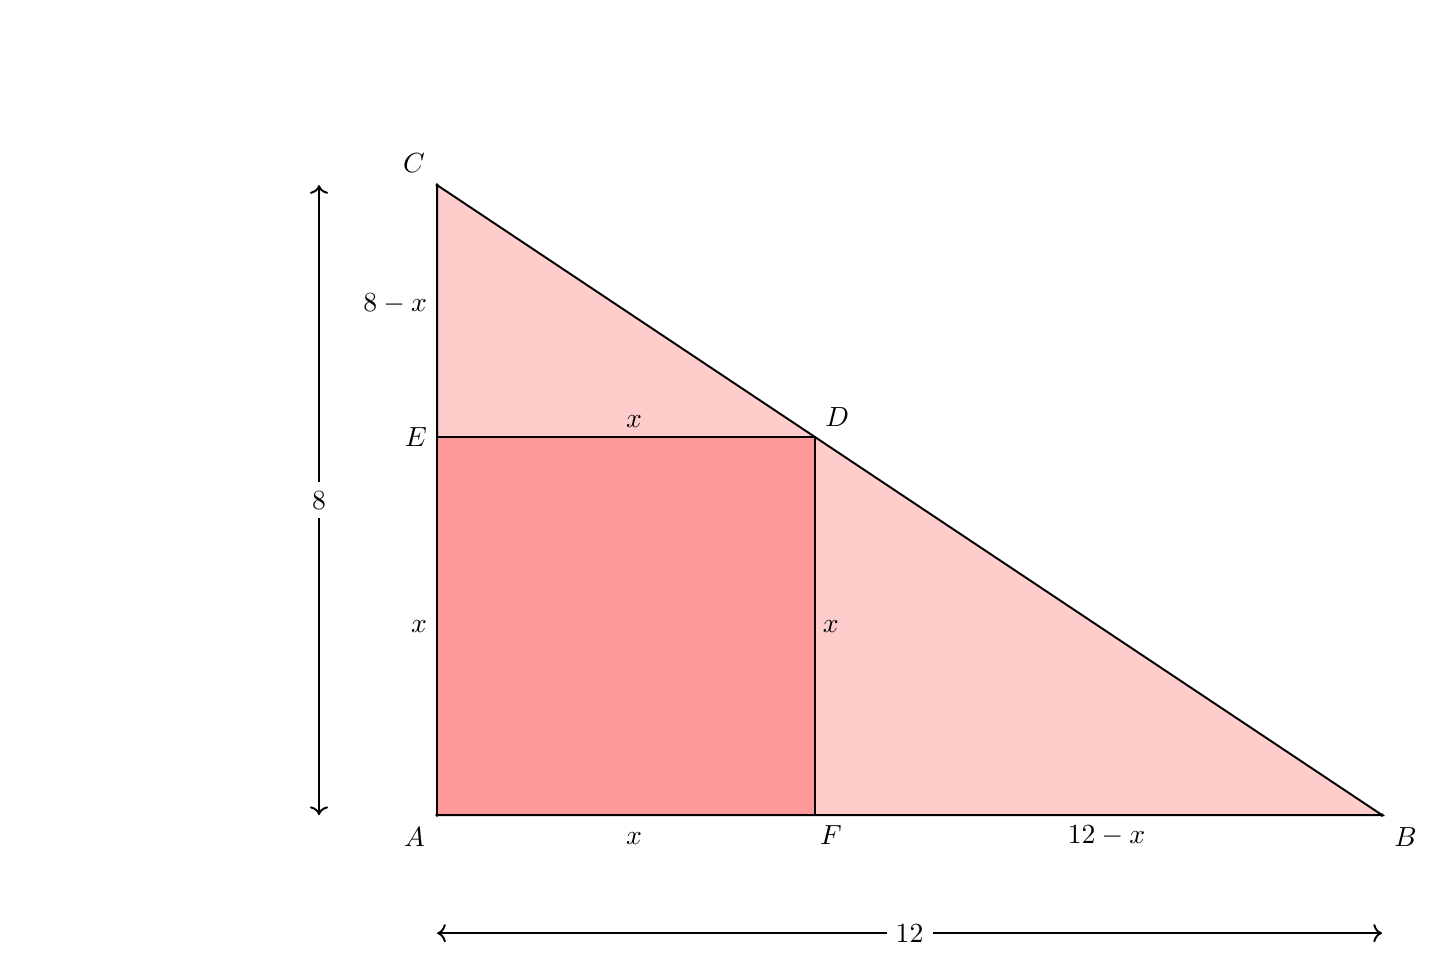
\begin{tikzpicture}[dot/.style={fill,circle,inner sep=.5pt},line width=.7pt]

%\draw[help lines,black!30] (-1,-1) grid (15.5,15.5);

\path 
  (0,0)  node[dot,label=below left:$A$]{} coordinate (A)
  (0,8)  node[dot,label=above left:$C$]{} coordinate (C)
  (12,0) node[dot,label=below right:$B$]{} coordinate (B);


% Desenhar o triângulo
\draw[fill=red!20] (A) -- (B) -- (C) -- cycle;
\draw[<->] ([xshift=-15mm]C) -- ([xshift=-15mm]A) node[midway,fill=white] {$8$};
\draw[<->] ([yshift=-15mm]A) -- ([yshift=-15mm]B) node[midway,fill=white] {$12$};
\path (8.5,0) node[below] {$12-x$};
\path (5,0) node[below] {$F$};

\path (0,6.5) node[left] {$8-x$};
\path (0,2.4) node[left] {$x$};
\path (2.5,5) node {$x$};
\path (5,2.4) node {$x$};
\path (2.5,-0.3) node {$x$};

\path[name path=CB] (C) -- (B);
\path[name path=AC] (A) -- (C);
\path[name path=Point] (A) -- (10,10);

\draw[fill=red!40,name intersections={of=CB and Point}] (0,0) rectangle (intersection-1) coordinate (x);

\path (x) node[above right] {$D$}; 
\path[name path=CBx] (x) -- +(-10,0);
\path[name intersections={of=CBx and AC}] (intersection-1) node[left] {$E$};

% Desenhar o quadrado

%\tkzMarkRightAngle(A,Q,P);
%\tkzMarkRightAngle(R,A,P);
%\tkzMarkAngle[size=0.75cm,color=cyan,mark=||](B,P,A);
%\tkzMarkAngle[size=1cm,color=cyan,mark=|](P,A,Q);

\end{tikzpicture}
\end{document}